%%%%%%%%%%%%%%%%%%%%%%%%%%%%%%%%%%%%%%%%%%%%%%%%%%%%%%%%%%%%%%%%%%%%%%%%%%%%
% AGUJournalTemplate.tex: this template file is for articles formatted with LaTeX
%
% This file includes commands and instructions
% given in the order necessary to produce a final output that will
% satisfy AGU requirements, including customized APA reference formatting.
%
% You may copy this file and give it your
% article name, and enter your text.
%
%
% Step 1: Set the \documentclass
%
%

%% To submit your paper:
\documentclass[draft]{agujournal2019}
\usepackage{url} %this package should fix any errors with URLs in refs.
\synctex=1

\usepackage{lineno}
\usepackage[finalnew]{trackchanges} %for better track changes. finalnew option will compile document with changes incorporated.
\usepackage{soul}
\linenumbers

\addeditor{bengoldman}
\addeditor{fasullo}

%%%%%%%
% As of 2018 we recommend use of the TrackChanges package to mark revisions.
% The trackchanges package adds five new LaTeX commands:
%
%  \note[editor]{The note}
%  \annote[editor]{Text to annotate}{The note}
%  \add[editor]{Text to add}
%  \remove[editor]{Text to remove}
%  \change[editor]{Text to remove}{Text to add}
%
% complete documentation is here: http://trackchanges.sourceforge.net/
%%%%%%%

%\draftfalse

%% Enter journal name below.
%% Choose from this list of Journals:
%
% JGR: Atmospheres
% JGR: Biogeosciences
% JGR: Earth Surface
% JGR: Oceans
% JGR: Planets
% JGR: Solid Earth
% JGR: Space Physics
% Global Biogeochemical Cycles
% Geophysical Research Letters
% Paleoceanography and Paleoclimatology
% Radio Science
% Reviews of Geophysics
% Tectonics
% Space Weather
% Water Resources Research
% Geochemistry, Geophysics, Geosystems
% Journal of Advances in Modeling Earth Systems (JAMES)
% Earth's Future
% Earth and Space Science
% Geohealth
%
% ie, \journalname{Water Resources Research}

\journalname{Geophysical Research Letters}


\begin{document}

%% ------------------------------------------------------------------------ %%
%  Title
%
% (A title should be specific, informative, and brief. Use
% abbreviations only if they are defined in the abstract. Titles that
% start with general keywords then specific terms are optimized in
% searches)
%
%% ------------------------------------------------------------------------ %%

% Example: \title{This is a test title}

\title{The Impact of Anthropogenic Forcing on ENSO Amplitude}

%% ------------------------------------------------------------------------ %%
%
%  AUTHORS AND AFFILIATIONS
%
%% ------------------------------------------------------------------------ %%

% Authors are individuals who have significantly contributed to the
% research and preparation of the article. Group authors are allowed, if
% each author in the group is separately identified in an appendix.)

% List authors by first name or initial followed by last name and
% separated by commas. Use \affil{} to number affiliations, and
% \thanks{} for author notes.
% Additional author notes should be indicated with \thanks{} (for
% example, for current addresses).

% Example: \authors{A. B. Author\affil{1}\thanks{Current address, Antartica}, B. C. Author\affil{2,3}, and D. E.
% Author\affil{3,4}\thanks{Also funded by Monsanto.}}

\authors{John Fasullo\affil{1}, Benjamin Goldman\affil{2}}


% \affiliation{1}{First Affiliation}
% \affiliation{2}{Second Affiliation}
% \affiliation{3}{Third Affiliation}
% \affiliation{4}{Fourth Affiliation}

\affiliation{1}{Climate and Global Dynamics Division, National Center for Atmospheric Research, 1850 Table Mesa Dr., Boulder, CO, USA}

\affiliation{2}{Science Research Program, White Plains High School, 550 North Street, White Plains, NY, USA}

%(repeat as many times as is necessary)

%% Corresponding Author:
% Corresponding author mailing address and e-mail address:

% (include name and email addresses of the corresponding author.  More
% than one corresponding author is allowed in this LaTeX file and for
% publication; but only one corresponding author is allowed in our
% editorial system.)

% Example: \correspondingauthor{First and Last Name}{email@address.edu}

\correspondingauthor{Benjamin Goldman}{bg502257@live.wpcsd.k12.ny.us}

%% Keypoints, final entry on title page.

%  List up to three key points (at least one is required)
%  Key Points summarize the main points and conclusions of the article
%  Each must be 140 characters or fewer with no special characters or punctuation and must be complete sentences

% Example:
% \begin{keypoints}
% \item	List up to three key points (at least one is required)
% \item	Key Points summarize the main points and conclusions of the article
% \item	Each must be 140 characters or fewer with no special characters or punctuation and must be complete sentences
% \end{keypoints}

\begin{keypoints}
\item NCAR's CESM Large Ensemble predicts increase to Ni\~{n}o 3.4 variance over the 21$^{st}$ century.
\item Increase can mainly be attributed to greenhouse gas and aerosol emissions.
\item Changes to ENSO amplitude are linked to changes to equatorial Pacific ocean stratification.
\end{keypoints}

%% ------------------------------------------------------------------------ %%
%
%  ABSTRACT and PLAIN LANGUAGE SUMMARY
%
% A good Abstract will begin with a short description of the problem
% being addressed, briefly describe the new data or analyses, then
% briefly states the main conclusion(s) and how they are supported and
% uncertainties.

% The Plain Language Summary should be written for a broad audience,
% including journalists and the science-interested public, that will not have 
% a background in your field.
%
% A Plain Language Summary is required in GRL, JGR: Planets, JGR: Biogeosciences,
% JGR: Oceans, G-Cubed, Reviews of Geophysics, and JAMES.
% see http://sharingscience.agu.org/creating-plain-language-summary/)
%
%% ------------------------------------------------------------------------ %%

%% \begin{abstract} starts the second page

\begin{abstract}

    The El Niño/Southern Oscillation (ENSO) is the dominant mode of interannual climate variability, with substantial associated global socio-economic impacts. Due to their significance, shifts in ENSO under climate change also have the potential to substantially impact human society and natural ecosystems. However, it is currently unclear what effect greenhouse gas (GHG) and industrial aerosol (AER) emissions have on ENSO, as well as what effect these factors have when combined. This study examined transient changes to ENSO variance under a variety of forcing scenarios using the CESM1 Large and Single-Forcing Ensembles. These multi-member ensembles span the historical record (1920-2005) and much of the 21st C (2006-2080 for GHG/AER). A 2000-year pre-industrial (PI) control simulation is used to account for model drift and 20-year running variance of the Niño 3.4 SST index is used as a proxy for ENSO variance. The ensemble mean and standard error of each ensemble was calculated, while the Probability Density Function (PDF) is computed for the PI control simulation to estimate the statistical significance of simulated changes. We calculated the correlation coefficient between ocean temperature in the equatorial Pacific and Ni\~{n}o 3.4 under various forcing conditions, concluding that Pacific stratification likely is tied to changes to ENSO amplitude. We identifed significant increases in variance of the Ni\~{n}o 3.4 index under full-forcing conditions during the historical record and attribute these mainly to changes in GHG, with the potential emergence of AER-driven increases in the decades to come. 

\end{abstract}

%\section*{Plain Language Summary}

%[ enter your Plain Language Summary here or delete this section]


%% ------------------------------------------------------------------------ %%
%
%  TEXT
%
%% ------------------------------------------------------------------------ %%

%%% Suggested section heads:
% \section{Introduction}
%
% The main text should start with an introduction. Except for short
% manuscripts (such as comments and replies), the text should be divided
% into sections, each with its own heading.

% Headings should be sentence fragments and do not begin with a
% lowercase letter or number. Examples of good headings are:

% \section{Materials and Methods}
% Here is text on Materials and Methods.
%
% \subsection{A descriptive heading about methods}
% More about Methods.
%
% \section{Data} (Or section title might be a descriptive heading about data)
%
% \section{Results} (Or section title might be a descriptive heading about the
% results)
%
% \section{Conclusions}


\section{Introduction}

\note[bengoldman]{problem/entity}El Ni\~{n}o is the main mode of interanual climate variability, originating from an interaction between the atmosphere and water movement and temperature in the Pacific ocean \cite{bjerknes1969atmospheric}. The reasons for studying ENSO are clear, as ENSO has drastically affected climate patterns worldwide, modulating rainfall and temperature in nearly every continent \cite{ropelewski1987global}. For example, the recent 2015-2016 El Ni\~{n}o event contributed to record-breaking high temperatures and droughts in South America \cite{jimenez2016record}. At the same time, long-term anthropogenic greenhouse gas emissions are causing global temperatures to increase through a greenhouse effect. The effect of greenhouse emissions and other factors on ENSO intensity remains unclear.

The two major ways in which the earth's climate varies are climate change and climate variability. Climate change is defined as climate changes caused by external factors, most notably greenhouse gasses, natural and artificial aerosol emissions, land use changes, and stratospheric ozone changes. Greenhouse gas emissions have a clear impact on the earth's climate, global warming. Climate change is usually long-term. In contrast, internal variability is defined as changes to the earth's climate originating from natural climatic processes, such as ENSO, Pacific Decadal Oscillation (PDO), Atlantic Multidecadal Oscillation (AMO), and others. Climate variability occurs on much shorter timescales, and is usually cyclical and driven by feedback loops.

\note[bengoldman]{focus on future experiments, describe results of literature, not methods} \note[bengoldman]{past research} Research on the effect of external forcing on ENSO remains inconclusive, as results from similar studies conflict. \citeA{nowack2017role} predicted an overall increase in Ni\~{n}o 3.4 standard deviation under a combination of 4xCO$_2$ and interactive ozone forcing using single-model simulations, showing that greenhouse gasses increase the frequency of extreme ENSO by favoring a more Ni\~{n}o-like in the tropical Pacific, while ozone dampens this effect. In contrast, a few studies have found that ENSO amplitude decreases under global warming in certain coupled models \cite{kohyama2018weakening}.

However, other studies have failed to find any statistically significant ENSO response to external forcing \cite{stevenson2012significant}. Analysis using NCAR's CESM Large Ensemble shows an ensemble size of at least 15 models is necessary to attribute changes to Ni\~{n}o variance to external forcing and reject the null hypothesis that internal variability is responsible for changes to ENSO \cite{zheng2018response}. Several modes of internal variability have been shown to modulate ENSO, including the AMO \cite{levine2017impact} and Tropical Pacific Decadal Variability (TPDV) \cite{zheng2018response}. An analysis of the Max Plank Institute's Grand Ensemble as well as NCAR's CESM Large Ensemble suggests that 80\% of changes to ENSO amplitude can be attributed to internal variability, but given a large enough ensemble, significant changes in ENSO amplitude due to climate change can be detected \cite{maher2018enso}.

In this study, we show that NCAR's CESM predicts significant increase in ENSO amplitude in the 21st century, and that greenhouse gasses and aerosol emissions play important roles in causing this increase. As in previous studies, the role of internal variability in conjunction with forcing was examined. We hypothesized that increased stratification in the future plays a large role in causing this predicted increase.

\section{Data}

The primary data source for this study is NCAR's Community Earth System Model Large Ensemble and Single Forcing Ensemble (CESM1-LE). The Large Ensemble contains 40 simulations of the CESM1 coupled model, forced with historic radiative forcing from 1920 to 2005 and according to the RCP 8.5 protocol from 2006 to 2100 \cite{kay2015community}. The single forcing ensemble is a collection of sub-ensembles for various climate factors (greenhouse gas, aerosols, biomass burning, land use, ozone). Each simulation is forced by a combination of all factors except for one, allowing the impact of a single factor to be deduced by subtracting the ensemble mean from the fully-forced ensemble mean \cite{deser2020isolating}. For example, the xghg (greenhouse gas) ensemble is forced by aerosol emissions, biomass burning, land use, and ozone. There is also a preindustrial control simulation, with all radiative forcing fixed at 1850 levels. 

\section{Methods and Results}
%% yay

\subsection{Ni\~{n}o 3.4 Variance}
We estimate 20th and 21st century ENSO amplitude for each model in the fully-forced, single-forced, and PI control CESM1 ensembles using the variance of the Ni\~{n}o 3.4 region of the Pacific ocean (5N-5S, 170W-120W). We measure variance on 20-year centered sliding windows. We calculate the multi-model mean for each ensemble, as well as the ensemble standard error. The results of this calculation are shown in figure \ref{fig:variance_1}.

The fully-forced ensemble exhibits moderate increase in variance, with the other ensembles showing less meaningful changes. In the fully-forced ensemble, the variance of the Ni\~{n}o 3.4 region increases beyond 2 standard errors of the control, increasing until the mid-21st century, and then decreasing gradually. The excluded greenhouse, aerosol, and biomass-burning ensembles also contain a slight increase, which may not be statistically significant. Although the excluded land use ensemble mean has a strong increase in variance, this result is unlikely to be meaningful due to the xlulc ensemble's low sample size. Additionally, all ensembles exhibit considerable noise, in line with previous studies \cite{maher2018enso}. 

\begin{figure}
    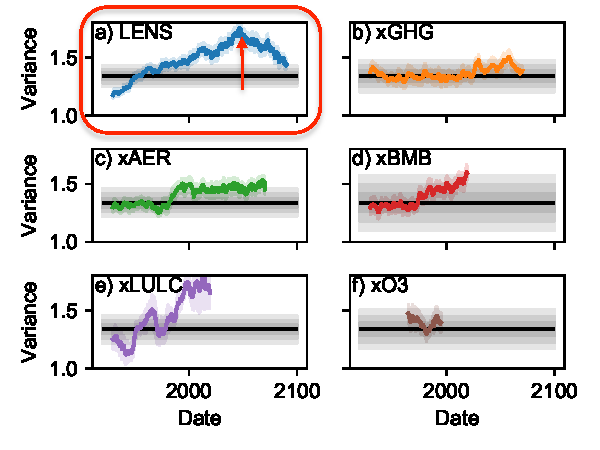
\includegraphics{figures/variance_1.pdf}
    \caption{20-year windowed variance of the Ni\~{n}o 3.4 region SST, for ensembles a) full-forcing, b) xghg, c) xaer, d) xbmb, e) xlulc, f) fixedO3. Grey bars are PI control mean and 1x, 2x, 3x standard error. Colored bars represent ensemble standard error.}
    \label{fig:variance_1}
\end{figure}

The fully-forced ensemble exhibits reduced variance in the mid-late 20th century, below that of the PI control. The most likely explanation for this phenomenon is internal variability. To test the likelihood of this explanation, we test the influence of the Atlantic Multidecadal Oscillation (AMO) and Atlantic Meridional Overturning Current (AMOC) on ENSO in the control simulation. The AMO has been shown to have an influence on ENSO strength and seasonal growth rate \cite{levine2017impact}. We filter the control Ni\~{n}o 3.4 variance data according to the strength of the AMO and AMOC, using records of AMO/C strength in the Climate Variability Diognostics Package (CVDP) \cite{phillips2014evaluating}. The Probability Distribution Function of Ni\~{n}o 3.4 variance is estimated for AMO/C > 1/2$\sigma$ and < -1/-2$\sigma$ using a Kernel Density Estimation. No meaningful differences were found in the distribution of ENSO intensity under any of these conditions (See Suplementary information figure 1).

\subsection{Single Forcing Scenarios and the Bootstrap Process}
We analyze the role of individual factors using the CESM Single Forcing Ensembles. To separate the influence of a single factor from the fully-forced ensemble, we employ a bootstrap test. For each single-forcing ensemble, a single simulation is randomly selected, and the Ni\~{n}o 3.4 20-year variance record is subtracted from that from a randomly selected fully-forced simulation. We repeat this process 1000 times for each ensemble, and then calculate the mean and standard error for each ensemble. These results are shown in figure \ref{fig:bootstrap_1}. The greenhouse-only ensemble as well as the aerosol-only ensemble exhibit increased variance, signaling that greenhouse and aerosol emissions likely both play a significant role in ENSO's forced response in the full-forcing ensemble. Interestingly, the influence of greenhouse gasses and aerosols are non-conflicting, in contrast with previous studies that show opposite effects of greenhouse gas and aerosol forcing on ENSO \cite{stevenson2019forced}. All the other single forcing ensembles exhibit insignificant differences from the fully-forced ensemble. The biomass burning case shows very small deviations from the fully-forced case, while the ozone ensemble's period of recording is too small to draw meaningful conclusions. However, \citeA{nowack2017role} showed that ozone forcing may dampen the effect of greenhouse-forced increases to ENSO amplitude by reducing changes to Pacific sea temperature and the Walker Circulation. The land use/cover case, while it does show large deviations from the fully-forced case, has an ensemble size (5 members) too small to lend any credibility to these changes.

\begin{figure}
    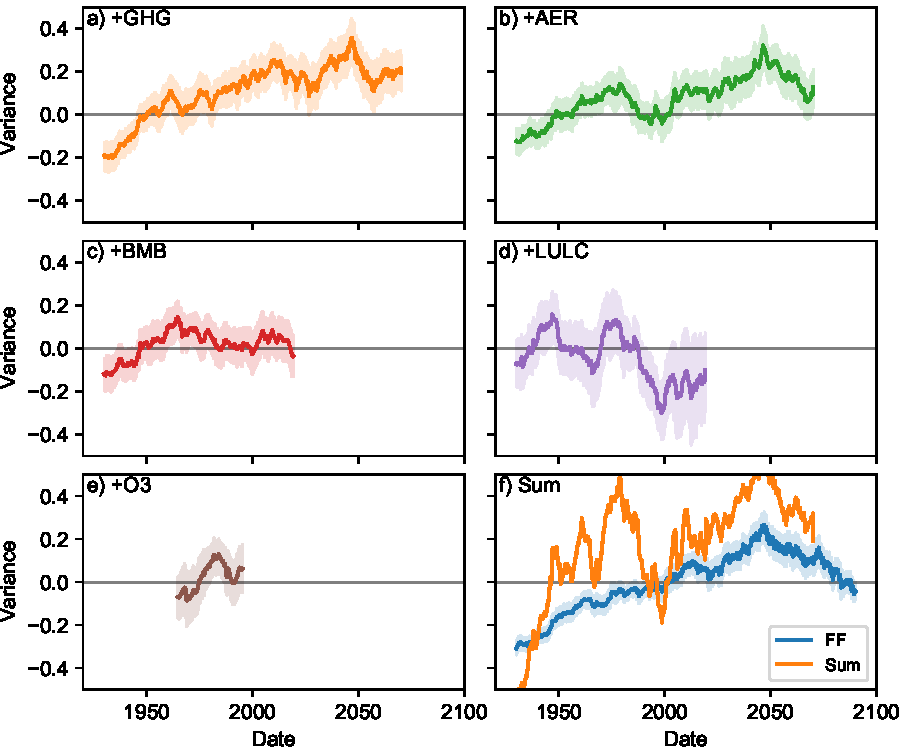
\includegraphics{figures/bootstrap_1.pdf}
    \caption{Difference between fully forced and single forced ensembles derived from the bootstrap process for a) greenhouse gas, b) aerosol emissions c) biomass burning, d) land use/cover, e) ozone; f) compares the sum of the bootstrapped ensemble means for the single forcing ensembles (blue) and the ensemble mean for the full forcing ensemble, detrended by a constant to center on zero (orange).}
    \label{fig:bootstrap_1}
\end{figure}

In both the fully-forced scenario, and the greenhouse and aerosol only simulations, there is noticeably reduced Ni\~{n}o 3.4 variance in the mid-20\^{th} century, below 2 standard errors of the control. We hypothesize that this discrepancy may be the result of anomalous initial conditions caused by internal variability of the control, as the control conditions are used to initialize all the forced runs. To test this hypothesis, we analyzed the impact of the Atlantic Multidecadal Oscillation (AMO) and the Atlantic Meridional Overturning Current (AMOC) on Ni\~{n}o 3.4 variance in the control simulation using records of the AMO and AMOC from the Climate Variability Diagnostics Package (CVDP) \cite{phillips2014evaluating}. We filtered the 20-year variance of the Ni\~{n}o 3.4 sea surface temperature in the control based on the strength of the AMO/AMOC, separating ENSO variance into groups where AMO < -1$\sigma$, AMO < -2$\sigma$, AMO > 1$\sigma$, AMO >2$\sigma$, and the same for AMOC. We then estimated the probability density function for each group using a kernel density estimator. We observed no consistent difference in the distribution of Ni\~{n}o 3.4 variance between any group. So far the question of reduced variance is unanswered, and it will be addressed in further depth later in the study.

\subsection{Correlation With Ocean Temperature}
Next, we analyzeed the correlation between ENSO amplitude and changes to ocean structure in the CESM1 ensembles. To do this we used 4 slices of ocean temperature from the fully-forced, xghg, and xaer ensembles, including a slice averaged along the equator and slices through the western, central, and eastern Pacific basins. We linearly detrend and smooth with a 30-year windowed mean the timeseries at each gridpoint and the Ni\~{n}o 3.4 variance. Next, we calculated the Pearson's correlation coefficient between each gridpoint and the Ni\~{n}o 3.4 variance timeseries. The correlation coefficients for the equatorial slice are shown in figure \ref{fig:tempdt_1}, and for the central slice in figure \ref{fig:tempcep_1}.

Overall, the majority of the Pacific basin exhibits negative correlation with Ni\~{n}o 3.4 variance when linearly detrended and smoothed. The fully-forced simulation contains strongly negative correlation between the subsurface layer of the equatorial Pacific and ENSO amplitude, leading to the hypothesis that forced changes to Pacific Ocean stratification may be connected to ENSO intensity. However, it is unclear whether there is also a causal relationship between the two. Additionally, it is unclear whether the overall warming trend of the upper Pacific ocean is connected to changes to ENSO intensity. We notice that the high levels of correlation between the subsurface layer and Ni\~{n}o 3.4 variance are present in the xGHG and xAER ensembles, as well as the fully forced ensemble, suggesting that there is a relationship between ENSO amplitude and subsurface Pacific Ocean temperature in a variety of forcing scenarios.

\begin{figure}
    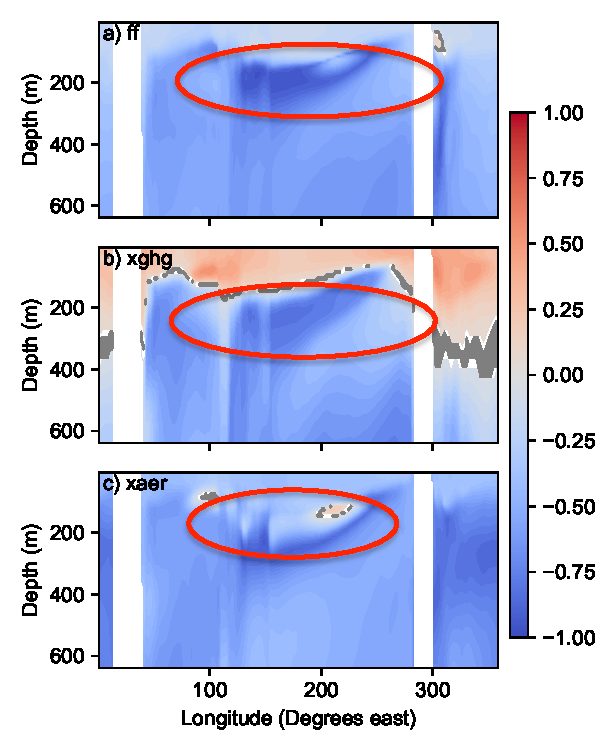
\includegraphics{figures/tempdt.pdf}
    \caption{Correlation coefficient between detrended and smoothed ocean temperature averaged along the equator and detrended and smoothed Ni\~{n}o 3.4 variance. Grey color indicates points where p<0.05. The white regions at 25 and 280 degrees East are Africa and South America.}
    \label{fig:tempdt_1}
\end{figure}


\begin{figure}
    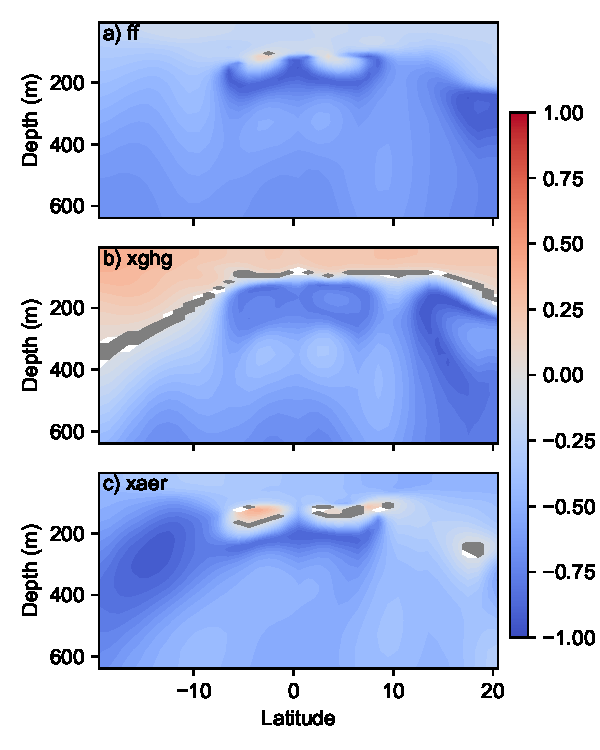
\includegraphics{figures/tempcep.pdf}
    \caption{Correlation coefficient between detrended and smoothed ocean temperature of the central pacific slice and detrended and smoothed Ni\~{n}o 3.4 variance. Grey color indicates points where p<0.05.}
    \label{fig:tempcep_1}
\end{figure}


\section{Conclusions and Discussion}
%% yay

In this study, predicted changes to ENSO amplitude are examined in the CESM1 Large Ensemble and Single Forcing Ensemble. The fully-forced large ensemble exhibits increased ENSO amplitude, as measured by calculating the 20-year variance of the Ni\~{n}o 3.4 index. These changes appear to be statistically significant, but need to be scrutinized further, as they are in disagreement with results of some previous studies \cite{stevenson2012significant}. Additionally, the fully-forced ensemble, as well as all the others contains considerable noise, as the individual members cover a wide range of variability. Greenhouse gas and aerosol emissions are likely the most significant contributors to these forced changes, as shown by the fact that the ensemble mean for the xGHG and xAER ensembles are the most different from the fully-forced mean. All the other single-forcing ensembles had insignificant differences from the fully forced ensemble, or were lacking a sample size large enough to lend credibility to their results. Analysis of the correlation coefficient between ENSO amplitude and Pacific ocean temperature reveals that changes to ENSO intensity are tied to changes to the subsurface layer of the tropical Pacific Ocean. It is still unclear what is driving this connection, as well as how external forcing such as global warming affects it. There has been shown to be a connection between Pacific stratification and ENSO variability as higher levels of stratification result in a stronger thermocline feedback, which causes the Pacific to become less stable, making strong ENSO events more likely \cite{dewitte2013reinterpreting}.

This study produced similar results as of previous studies, as it predicts an increase in ENSO amplitude, as well as overwhelming noise caused by internal variability \cite{maher2018enso}. Although there is limited research on the impact of individual external factors on ENSO, this study complements the results of \citeA{stevenson2019forced}, who observed conflicting effects of greenhouse gas and aerosol emissions on ENSO diversity. In contrast, this study observes that the impact on ENSO amplitude of greenhouse gas and aerosols has the same sign. This result is also surprising given that greenhouse and aerosol emissions have been shown to have opposite effects on sea surface temperature and global circulation, with greenhouse emissions favoring a more Ni\~{n}o-like state with weakened Walker circulation and higher SST, and aerosol emissions counteracting these effects \cite{boer2000transient}.

This study has a number of goals for future continuation. The most pressing of these goals is a deeper analysis of changes to Pacific Ocean structure, which will be done by examining correlation between ENSO amplitude and potential density, as well as comparisons of changes to stratification in the Pacific. Additionally, the methods of this study will be repeated on the CESM2 large ensemble, which has a larger ensemble size and a longer record period, as compared to CESM1. Analysis of the CMIP6 models are also necessary to verify these results across variations in model physics. Deeper statistical analyses of changes to ENSO amplitude should also be tone to further examine the likelihood and intensity of future changes to ENSO amplitude. Lastly, correlation between ENSO amplitude and internal variability should be further investigated using the records provided by the CVDP. Doing these further analyses will help to verify the results of this study, while more precisely analyzing future changes to ENSO.

The results of this study will help to direct future studies on the impact of climate change on ENSO by providing one further data point supporting the conclusion that ENSO will intensify due to global warming. This study and others like it will help societies impacted by ENSO to prepare for intensification in the future.

%%

%  Numbered lines in equations:
%  To add line numbers to lines in equations,
%  \begin{linenomath*}
%  \begin{equation}
%  \end{equation}
%  \end{linenomath*}



%% Enter Figures and Tables near as possible to where they are first mentioned:
%
% DO NOT USE \psfrag or \subfigure commands.
%
% Figure captions go below the figure.
% Table titles go above tables;  other caption information
%  should be placed in last line of the table, using
% \multicolumn2l{$^a$ This is a table note.}
%
%----------------
% EXAMPLE FIGURES
%
% \begin{figure}
% 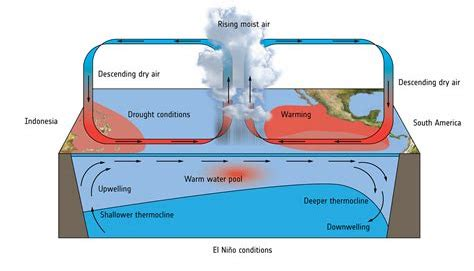
\includegraphics{example.png}
% \caption{caption}
% \end{figure}
%
% Giving latex a width will help it to scale the figure properly. A simple trick is to use \textwidth. Try this if large figures run off the side of the page.
% \begin{figure}
% \noindent\includegraphics[width=\textwidth]{anothersample.png}
%\caption{caption}
%\label{pngfiguresample}
%\end{figure}
%
%
% If you get an error about an unknown bounding box, try specifying the width and height of the figure with the natwidth and natheight options. This is common when trying to add a PDF figure without pdflatex.
% \begin{figure}
% \noindent\includegraphics[natwidth=800px,natheight=600px]{samplefigure.pdf}
%\caption{caption}
%\label{pdffiguresample}
%\end{figure}
%
%
% PDFLatex does not seem to be able to process EPS figures. You may want to try the epstopdf package.
%

%
% ---------------
% EXAMPLE TABLE
%
% \begin{table}
% \caption{Time of the Transition Between Phase 1 and Phase 2$^{a}$}
% \centering
% \begin{tabular}{l c}
% \hline
%  Run  & Time (min)  \\
% \hline
%   $l1$  & 260   \\
%   $l2$  & 300   \\
%   $l3$  & 340   \\
%   $h1$  & 270   \\
%   $h2$  & 250   \\
%   $h3$  & 380   \\
%   $r1$  & 370   \\
%   $r2$  & 390   \\
% \hline
% \multicolumn{2}{l}{$^{a}$Footnote text here.}
% \end{tabular}
% \end{table}

%% SIDEWAYS FIGURE and TABLE
% AGU prefers the use of {sidewaystable} over {landscapetable} as it causes fewer problems.
%
% \begin{sidewaysfigure}
% \includegraphics[width=20pc]{figsamp}
% \caption{caption here}
% \label{newfig}
% \end{sidewaysfigure}
%
%  \begin{sidewaystable}
%  \caption{Caption here}
% \label{tab:signif_gap_clos}
%  \begin{tabular}{ccc}
% one&two&three\\
% four&five&six
%  \end{tabular}
%  \end{sidewaystable}

%% If using numbered lines, please surround equations with \begin{linenomath*}...\end{linenomath*}
%\begin{linenomath*}
%\begin{equation}
%y|{f} \sim g(m, \sigma),
%\end{equation}
%\end{linenomath*}

%%% End of body of article

%%%%%%%%%%%%%%%%%%%%%%%%%%%%%%%%
%% Optional Appendix goes here
%
% The \appendix command resets counters and redefines section heads
%
% After typing \appendix
%
%\section{Here Is Appendix Title}
% will show
% A: Here Is Appendix Title
%
%\appendix
%\section{Here is a sample appendix}

%%%%%%%%%%%%%%%%%%%%%%%%%%%%%%%%%%%%%%%%%%%%%%%%%%%%%%%%%%%%%%%%
%
% Optional Glossary, Notation or Acronym section goes here:
%
%%%%%%%%%%%%%%
% Glossary is only allowed in Reviews of Geophysics
%  \begin{glossary}
%  \term{Term}
%   Term Definition here
%  \term{Term}
%   Term Definition here
%  \term{Term}
%   Term Definition here
%  \end{glossary}

%
%%%%%%%%%%%%%%
% Acronyms
%   \begin{acronyms}
%   \acro{Acronym}
%   Definition here
%   \acro{EMOS}
%   Ensemble model output statistics
%   \acro{ECMWF}
%   Centre for Medium-Range Weather Forecasts
%   \end{acronyms}

%
%%%%%%%%%%%%%%
% Notation
%   \begin{notation}
%   \notation{$a+b$} Notation Definition here
%   \notation{$e=mc^2$}
%   Equation in German-born physicist Albert Einstein's theory of special
%  relativity that showed that the increased relativistic mass ($m$) of a
%  body comes from the energy of motion of the body—that is, its kinetic
%  energy ($E$)—divided by the speed of light squared ($c^2$).
%   \end{notation}




%%%%%%%%%%%%%%%%%%%%%%%%%%%%%%%%%%%%%%%%%%%%%%%%%%%%%%%%%%%%%%%%
%
%  ACKNOWLEDGMENTS
%
% The acknowledgments must list:
%
% >>>>	A statement that indicates to the reader where the data
% 	supporting the conclusions can be obtained (for example, in the
% 	references, tables, supporting information, and other databases).
%
% 	All funding sources related to this work from all authors
%
% 	Any real or perceived financial conflicts of interests for any
%	author
%
% 	Other affiliations for any author that may be perceived as
% 	having a conflict of interest with respect to the results of this
% 	paper.
%
%
% It is also the appropriate place to thank colleagues and other contributors.
% AGU does not normally allow dedications.


\acknowledgments



%% ------------------------------------------------------------------------ %%
%% References and Citations

%%%%%%%%%%%%%%%%%%%%%%%%%%%%%%%%%%%%%%%%%%%%%%%
%
% \bibliography{<name of your .bib file>} don't specify the file extension
%
% don't specify bibliographystyle
%%%%%%%%%%%%%%%%%%%%%%%%%%%%%%%%%%%%%%%%%%%%%%%

\bibliography{references.bib}
This material is based upon work supported by the National Center for Atmospheric Research, which is a major facility sponsored by the National Science Foundation under Cooperative Agreement No. 1852977. Computing resources (doi:10.5065/D6RX99HX) were provided by the Climate Simulation Laboratory at NCAR's Computational and Information Systems Laboratory, sponsored by the National Science Foundation and other agencies. I would like to thank Ms. Kimberly Fleming and the White Plains High School Science Research Program for providing support in this study.


%Reference citation instructions and examples:
%
% Please use ONLY \cite and \citeA for reference citations.
% \cite for parenthetical references
% ...as shown in recent studies (Simpson et al., 2019)
% \citeA for in-text citations
% ...Simpson et al. (2019) have shown...
%
%
%...as shown by \citeA{jskilby}.
%...as shown by \citeA{lewin76}, \citeA{carson86}, \citeA{bartoldy02}, and \citeA{rinaldi03}.
%...has been shown \cite{jskilbye}.
%...has been shown \cite{lewin76,carson86,bartoldy02,rinaldi03}.
%... \cite <i.e.>[]{lewin76,carson86,bartoldy02,rinaldi03}.
%...has been shown by \cite <e.g.,>[and others]{lewin76}.
%
% apacite uses < > for prenotes and [ ] for postnotes
% DO NOT use other cite commands (e.g., \citet, \citep, \citeyear, \nocite, \citealp, etc.).
%



\end{document}


\section*{extra stuff}

More Information and Advice:

%% ------------------------------------------------------------------------ %%
%
%  SECTION HEADS
%
%% ------------------------------------------------------------------------ %%

% Capitalize the first letter of each word (except for
% prepositions, conjunctions, and articles that are
% three or fewer letters).

% AGU follows standard outline style; therefore, there cannot be a section 1 without
% a section 2, or a section 2.3.1 without a section 2.3.2.
% Please make sure your section numbers are balanced.
% ---------------
% Level 1 head
%
% Use the \section{} command to identify level 1 heads;
% type the appropriate head wording between the curly
% brackets, as shown below.
%
%An example:
%\section{Level 1 Head: Introduction}
%
% ---------------
% Level 2 head
%
% Use the \subsection{} command to identify level 2 heads.
%An example:
%\subsection{Level 2 Head}
%
% ---------------
% Level 3 head
%
% Use the \subsubsection{} command to identify level 3 heads
%An example:
%\subsubsection{Level 3 Head}
%
%---------------
% Level 4 head
%
% Use the \subsubsubsection{} command to identify level 3 heads
% An example:
%\subsubsubsection{Level 4 Head} An example.
%
%% ------------------------------------------------------------------------ %%
%
%  IN-TEXT LISTS
%
%% ------------------------------------------------------------------------ %%
%
% Do not use bulleted lists; enumerated lists are okay.
% \begin{enumerate}
% \item
% \item
% \item
% \end{enumerate}
%
%% ------------------------------------------------------------------------ %%
%
%  EQUATIONS
%
%% ------------------------------------------------------------------------ %%

% Single-line equations are centered.
% Equation arrays will appear left-aligned.

Math coded inside display math mode \[ ...\]
 will not be numbered, e.g.,:
 \[ x^2=y^2 + z^2\]

 Math coded inside \begin{equation} and \end{equation} will
 be automatically numbered, e.g.,:
 \begin{equation}
 x^2=y^2 + z^2
 \end{equation}


% To create multiline equations, use the
% \begin{eqnarray} and \end{eqnarray} environment
% as demonstrated below.
\begin{eqnarray}
  x_{1} & = & (x - x_{0}) \cos \Theta \nonumber \\
        && + (y - y_{0}) \sin \Theta  \nonumber \\
  y_{1} & = & -(x - x_{0}) \sin \Theta \nonumber \\
        && + (y - y_{0}) \cos \Theta.
\end{eqnarray}

%If you don't want an equation number, use the star form:
%\begin{eqnarray*}...\end{eqnarray*}

% Break each line at a sign of operation
% (+, -, etc.) if possible, with the sign of operation
% on the new line.

% Indent second and subsequent lines to align with
% the first character following the equal sign on the
% first line.

% Use an \hspace{} command to insert horizontal space
% into your equation if necessary. Place an appropriate
% unit of measure between the curly braces, e.g.
% \hspace{1in}; you may have to experiment to achieve
% the correct amount of space.


%% ------------------------------------------------------------------------ %%
%
%  EQUATION NUMBERING: COUNTER
%
%% ------------------------------------------------------------------------ %%

% You may change equation numbering by resetting
% the equation counter or by explicitly numbering
% an equation.

% To explicitly number an equation, type \eqnum{}
% (with the desired number between the brackets)
% after the \begin{equation} or \begin{eqnarray}
% command.  The \eqnum{} command will affect only
% the equation it appears with; LaTeX will number
% any equations appearing later in the manuscript
% according to the equation counter.
%

% If you have a multiline equation that needs only
% one equation number, use a \nonumber command in
% front of the double backslashes (\\) as shown in
% the multiline equation above.

% If you are using line numbers, remember to surround
% equations with \begin{linenomath*}...\end{linenomath*}

%  To add line numbers to lines in equations:
%  \begin{linenomath*}
%  \begin{equation}
%  \end{equation}
%  \end{linenomath*}



